\label{Chapter:Introduction:DL}

In order to be able to understand the chapters that will come later in this document, it is important to make a brief introduction of what \emph{Deep Learning}(DL) refers to. Deep learning is included in the field of Machine Learning, which is also included in the field of general Artificial Intelligence.

In Chapter \ref{Chapter:Intro:Rep:Learning}, an intuitive definition of what Machine Learning is was given. We said that ML studies the algorithms that improve from experience. Tom M. Mitchell \citep{mitchell_machine_1997} provided a more formal definition of what \emph{learning from experience} means:

\begin{ndefC}
A computer program is said to \emph{learn} from experience $E$ with respect some class of tasks $T$ and performance measure $P$, if its performance at tasks in $T$, as measured by $P$, improves with experience $E$.
\end{ndefC}

We would also like to have a DL definition. In \cite{deng_deep_2014}, multiple similar definitions are given. We present here the simplest of them:

\begin{ndefC}
\emph{Deep Learning} is a class of ML learning techniques that exploit many layers of non-linear information processing for supervised or unsupervised feature extraction and transformation, and for pattern analysis and classification.
\end{ndefC}

Usually, these techniques are based on the biologically inspired \emph{neural networks}(NNs), which consists in several connected units: the \emph{neurons}. Each neuron is basically a Perceptron, which is a is a weighted sum followed by a non-linear function, called an \emph{activator} in the ML context. Formally, the output of each neuron is 
\[
y = \phi\left(w_0 +\sum_{i = 1}^N w_i x_i \right) .   
\]
There are many activation functions, but the following examples must be remarked:
\begin{itemize}
\item Sigmoid. The sigmoid function is defined as follows:
\[
\phi(x) = \frac{1}{1+ e^{-x}}.
\]
This is one of the most common used activation functions. It is differentiable, monotonic and smooth. One of its main disadvantages is that at the right part of the function, the change in the values that the function takes converges to zero, so we get to the \emph{vanishing gradient} problem and the learning is minimal.

\begin{figure}[H]
    \centering
    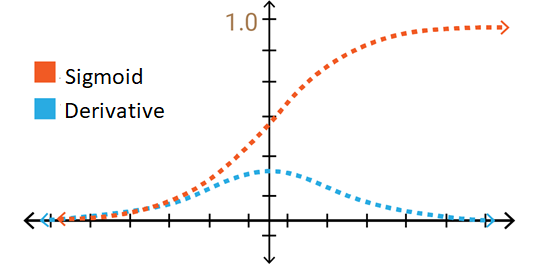
\includegraphics[width=0.5\linewidth]{sigmoid}
    \caption{Sigmoid. Image from \href{https://xzz201920.medium.com/activation-functions-linear-non-linear-in-deep-learning-relu-sigmoid-softmax-swish-leaky-relu-a6333be712ea}{this Medium article}. } \label{fig:sigmoid}
\end{figure}

\item Hyperbolic Tangent. This function is defined as follows:
\[
\phi(x) = \operatorname{tanh}(x) =  \frac{e^x - e^{-x}}{e^x + e^{-x}}.    
\]
This activation function has a small advantage over the sigmoid: its derivative is more steep, which means it can get more value and the learning can be more efficient.

\begin{figure}[H]
    \centering
    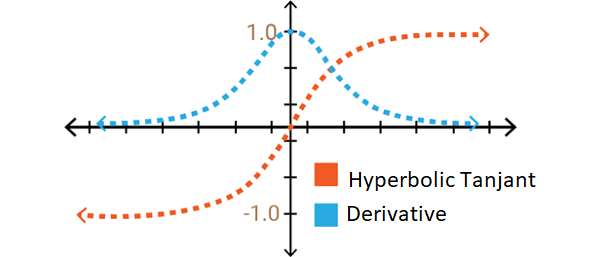
\includegraphics[width=0.6\linewidth]{tanh}
    \caption{Hyperbolic Tangent. Image from \href{https://xzz201920.medium.com/activation-functions-linear-non-linear-in-deep-learning-relu-sigmoid-softmax-swish-leaky-relu-a6333be712ea}{this Medium article}. } \label{fig:tanh}
\end{figure}

\item Rectified Linear Unit (ReLU). This function takes the following form:
\[
\phi(x) = \max\left(0,x\right).    
\]
ReLu is highly computationally efficient and non-linear. Its main problem is that when the inputs approach zero or are negative, the network can not perform back propagation and can not learn.

\begin{figure}[H]
    \centering
    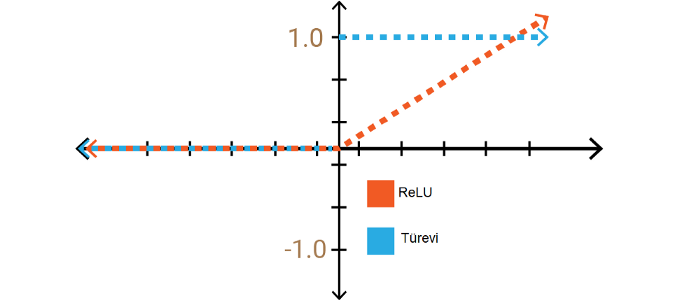
\includegraphics[width=0.6\linewidth]{relu}
    \caption{ReLU. Image from \href{https://xzz201920.medium.com/activation-functions-linear-non-linear-in-deep-learning-relu-sigmoid-softmax-swish-leaky-relu-a6333be712ea}{this Medium article}. } \label{fig:relu}
\end{figure}
\end{itemize}



\section{Neural Networks}

Using neurons and activation functions, we can formally define NNs. A NN with $L$ hidden layers is a deterministic non-linear function $f$, parametrized by a set of matrices $W = \{W_0,\cdots,W_L\}$ and non-linear activation functions $\{\phi_0,\cdots,\phi_L\}$. Given an input $x$, the output $y$ of the network is calculated as follows:
\[
h_0 = \phi_0\left(W_0^Tx\right), \cdots, h_l = \phi_l\left(W_l^T h_{l-1}\right),\cdots, y = \phi_L\left(W_L^T h_{L-1}\right).
\]
Having a NN, we consider it \emph{deep} when the number of hidden layers (and, consequently, the number of matrices) is considered high. 

Neural networks use loss functions, which define how well the output returned by the network matches the real output, reducing the learning problem to an optimization problem. The problem is finding $W^{\operatorname{opt}}$, such that
\[
W^{\operatorname{opt}}   = \argmin_{w} \sum_{n = 1}^N l(y_n, f_w(x_n)),
\]
where $\mathcal D = \{(x_n,y_n)\}$ is a dataset.

This problem is solved using a variant of \emph{stochastic gradient descent (SGD)}. This algorithm involves the computation of the loss function derivatives respect to the network parameters, and updates the parameters using this derivatives. Specifically, the parameters are updated as follows:
\[
W_{t+1} = W_t + \eta \nabla f(W_t),
\]
where $\eta \in \R^+$ is a small constant called the \emph{learning rate}. This algorithm guarantees convergence to local minimums of $f$ and, if $f$ is convex, the algorithm converges to a global minimum.

The last comment about neural networks is that, since the weights $W = \{W_0,\cdots,W_L\}$ are constantly updated, the derivatives have to be computed repeatedly. The computational cost of this is quite high. \emph{Backpropagation} was born to calculate the derivatives of the weights much faster. The intuitive idea is that the gradient of the layer $l$ is computed using the gradient of the layer $l+1$ using the chain rule.

Understanding both SGD and Backpropagation is crucial for understanding how NNs  work. However, in the experimentation part of this work we will focus on researching how a few hyperparameters affect the results of the proposed frameworks, so no further explanation on these important concepts will be provided.

\section{Convolutional Neural Networks}

Convolutional Neural Networks (CNNs) are a specific type of Neural Networks. The difference that we have between CNNs and NNs is that CNNs assume that the inputs have local dependencies. For instance, using an image, a CNN assumes (most of the time correctly) that given a pixel $x_{ij}$ of an input $x$, the neighbours of this pixels will have similar values or intensities. This allows us to encode certain properties into the architecture of the network.

If we use colored images, the input of the CNNs are 3-dimensional volumes, which will be transformed in some layers to other 3-dimensional volumes. In order to do this we have different types of layers, remarking \emph{convolutional} layers, \emph{pooling} layers and \emph{fully connected} layers. The most important ones are convolutional layers.

Convolutional layers receive a \emph{tensor} with shape $k \times n \times m \times c$, which means that the layer receives $k \in \mathbb N$ inputs of sizes $n \times m \times c$.  After the convolutional layer, the input has shape $k \times n' \times m' \times c'$, where $n'$ can be different from $n$ (respectively $m',c'$). One convolutional layer can apply one or several filters to the same input, producing different 2-dimensional activation maps that are stacked along the depth dimension to produce the output.

Formally, a convolution is the process of adding each element of the image to its local neighbours, weighted by a kernel. That is in our case performing a dot product between the input and the filter. We obtain
\[
g(x,y) = \omega \star f(x,y) = \sum_{dx = -a}^a \sum_{dy = -b}^b \omega(dx,dy)f(x+dx,y+dy),    
\]
where $g(x,y)$ is the pixel $(x,y)$ of the filtered image, $f(x,y)$ is the same pixel in the original image, and $\omega$ is the filter kernel. Depending on the filter kernel, the result will be different. 
\begin{nexample}
If we want to produce noise reduction in an image, we use Gaussian Blur, which kernel is calculated by a Gaussian function like the one in Equation \ref{gaussian:function}. For instance, a $3\times 3 $ gaussian kernel would approximately be:
\[
\frac{1}{16}\begin{bmatrix}
    1 & 2 & 1\\
    2 & 4 & 2\\
    1 & 2 & 1
\end{bmatrix}.
\]
\end{nexample}

\subsection{ResNet}

To finish with this introduction to CNNs, we will present a widely used CNN architecture. Since CNNs appeared, people tried to build such deep networks that were very hard to train. When deeper networks start converging, a degradation problem ocurred: with the network depth increasing, accuracy gets saturated and then it degraded rapidly. \emph{ResNet} \citep{he2015deep} brought and end to this problem, allowing the training of very deep models with up to hundreds of layers.

In the paper, they mentioned that if $\mathcal H(x)$ is the underlying map of a sequence of layers and knowing that it can be asymptotically approximated, we can also approximate its residuals
\[
\mathcal F(x) = \mathcal H(x) - x.    
\]
Then, the original function becomes $\mathcal F(x) + x$. In order to achieve this, they introduced the \emph{Residual Block}, a block of layers that introduces skip or shortcut connections that makes it easy for networks to represent the identity mapping. We can see one of this blocks depicted in Figure \ref{fig:resnet:block}.

\begin{figure}[H]
    \centering
    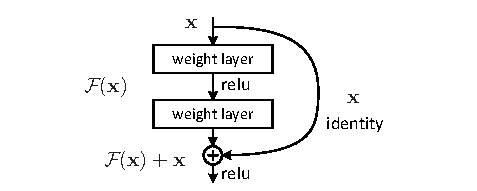
\includegraphics[width=0.6\linewidth]{block}
    \caption{Residual Block. Image from \cite{he2015deep} } \label{fig:resnet:block}
\end{figure}

Usually, ResNet comes accompanied by a number (e.g. \emph{Resnet-50}), that indicates the number of layers it has. Usually, a \emph{batch normalization} is used after each convolution and ReLU is used at the end of each group of layers.

\begin{table}[H]
    \label{arch:resnet:18}
    \centering
    \begin{tabular}{llc}
    Layers                      & Output Size                     & Resnet 18                                                                     \\ \hline
    $conv1$                     & $112\times112$                  & $7 \times 7, \ 64$, stride 2                                                  \\
    \multirow{2}{*}{$conv2\_x$} & \multirow{2}{*}{$56 \times 56$} & $3 \times 3$ max pool, stride 2                                               \\
                                &                                 & $\begin{bmatrix}3 \times 3 , & 64 \\ 3 \times 3,& 64 \end{bmatrix} \times 2$  \\
    $conv3\_x$                  & $28 \times 28$                  & $\begin{bmatrix} 3\times 3, & 128 \\ 3\times 3, & 128 \end{bmatrix} \times 2$ \\
    $conv4\_x$                  & $14 \times 14$                  & $\begin{bmatrix} 3\times 3, & 256\\ 3\times 3, & 256\end{bmatrix} \times 2$   \\
    $conv5\_x$                  & $7 \times 7$                    & $\begin{bmatrix} 3\times 3, & 512\\ 3\times 3, & 512\end{bmatrix} \times 2$   \\
                                & $1\times 1 $                    & average pool, 1000-d fc, softmax                                             
    \end{tabular}
    \caption{Resnet 18 architecture.}
    \end{table}

For instance, having a look at the Table \ref{arch:resnet:18}, in the convolution block \emph{conv\_2}, we have two convolutions 